\chapter{Casi d'uso}\label{sec:casi}
\section{Introduzione}
In questa sezione del documento vengono riportati tutti i casi d'uso relativi al prodotto del progetto.\\
Ogni caso d'uso sarà identificato da un codice alfanumerico, composto dall'acronimo "UC" di use case e seguito da dei numeri. Per ottenere una gerarchizzazione ad albero dei casi d'uso, con cui segnalare un sotto caso d'uso di un altro, i numeri saranno seguiti da uno o più punti, con cui sarà facile identificare il sotto caso d'uso rispetto al suo padre.\\
Ogni use case sarà inoltre corredato dalle informazioni riguardanti descrizione generale, \emph{attore\ped{G}} principale, pre condizioni, post condizioni e scenario, oltre ad attori secondari, generalizzazioni ed estensioni qualora presenti.

\section{Attori}
A seguito della richiesta esplicita da parte del proponente di non implementare alcun meccanismo di autenticazione, non vengono distinti nell'analisi dei casi d'uso utenti autenticati o meno, né utenti amministratori.\\
Per questo motivo, l'unico attore principale di tutti i casi d'uso sarà un utente generico, definito "user" negli UML dei casi d'uso.\\
L'attore secondario, definito con l'acronimo \ccgloss{LLM}, identifica il modello large language che è alla base del funzionamento del chatbot e delle funzionalità che permettono l'interazione dell'utente con esso. Il modello è identificato come attore secondario, e non come parte del sistema stesso, in quanto non sarà allenato dal sistema né il sistema avrà alcun potere su di esso.

\begin{figure}[H]
    \centering
    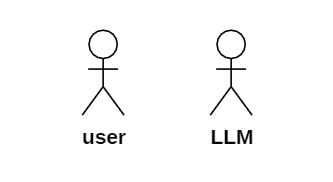
\includegraphics[width=0.4\linewidth]{Attori.PNG}
    \caption{Attori}
    \label{fig:attori}
\end{figure}

\newpage

\section{Elenco dei casi d'uso}

\subsection{UC-1 Visualizza lista documenti}
\begin{description}
    \item[Descrizione:] L’utente vuole visualizzare la lista dei documenti presenti nel sistema.
    \item[Attore primario:] Utente generico.
    \item[Pre condizioni:] Il sistema mostra l’interfaccia di gestione documenti.
    \item[Post condizioni:] Il sistema mostra l’intera lista di documenti.
    \item[Scenario:] 
    \begin{enumerate}
        \item[]
        \item L’utente visualizza la lista di tutti documenti.
    \end{enumerate}
\end{description}

\begin{figure}[H]
    \centering
    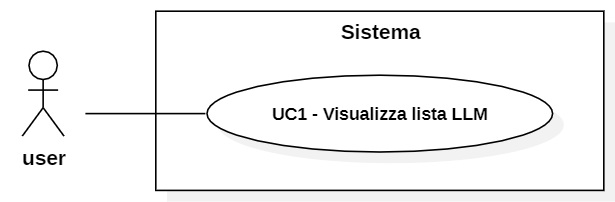
\includegraphics[width=0.8\linewidth]{UC1.PNG} %da modificare
    \caption{Diagramma UML del caso d'uso UC-1}
    \label{fig:UC3}
\end{figure}

\subsection{UC-1.1 Visualizza singolo documento}
\begin{description}
    \item[Descrizione:] L'utente vuole visualizzare un particolare documento presente nel sistema.
    \item[Attore primario:] Utente generico.
    \item[Pre condizioni:] Il sistema mostra l’intera lista di documenti.
    \item[Post condizioni:] Il sistema mostra il documento di interesse.
    \item[Scenario:]
    \begin{enumerate}
        \item[]
        \item L’utente visualizza la lista di tutti documenti (\textbf{UC-1}).
        \item L'utente visualizza il singolo documento.
    \end{enumerate} 
\end{description}

\begin{figure}[H]
    \centering
    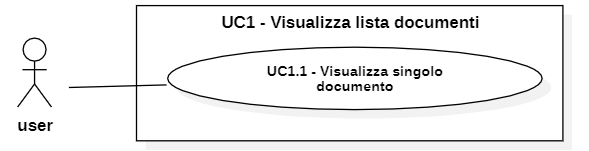
\includegraphics[width=0.8\linewidth]{UC1.1.PNG}
    \caption{Diagramma UML dei casi d'uso UC-1.1}
    \label{fig:UC3.1}
\end{figure}

\subsection{UC-1.1.1 Visualizza nome del documento}
\begin{description}
    \item[Descrizione:] L'utente vuole visualizzare il nome del documento di interesse.
    \item[Attore primario:] Utente generico.
    \item[Pre condizioni:] Il sistema mostra l’intera lista di documenti.
    \item[Post condizioni:] Il sistema mostra il nome del documento selezionato.
    \item[Scenario:]
    \begin{enumerate}
        \item[]
        \item L’utente visualizza la lista di tutti documenti (\textbf{UC-1}).
        \item L'utente visualizza il singolo documento (\textbf{UC-1.1}).
        \item L'utente visualizza il nome del documento.
    \end{enumerate} 
\end{description}

\subsection{UC-1.1.2 Visualizza data di inserimento del documento}
\begin{description}
    \item[Descrizione:] L'utente vuole visualizzare la data di inserimento del documento di interesse.
    \item[Attore primario:] Utente generico.
    \item[Pre condizioni:] Il sistema mostra l’intera lista di documenti.
    \item[Post condizioni:] Il sistema mostra la data di inserimento del documento selezionato.
    \item[Scenario:] 
    \begin{enumerate}
        \item[]
        \item L’utente visualizza la lista di tutti documenti (\textbf{UC-1}).
        \item L'utente visualizza il singolo documento (\textbf{UC-1.1}).
        \item L'utente visualizza la data di inserimento del documento voluto.
    \end{enumerate}
\end{description}

\subsection{UC-1.1.3 Visualizza tag del documento}
\begin{description}
    \item[Descrizione:] L'utente vuole visualizzare i tag applicati al documento di interesse.
    \item[Attore primario:] Utente generico.
    \item[Pre condizioni:] Il sistema mostra l’intera lista di documenti.
    \item[Post condizioni:] Il sistema mostra i tag del documento selezionato.
    \item[Scenario:]
    \begin{enumerate}
        \item[]
        \item L’utente visualizza la lista di tutti documenti (\textbf{UC-1}).
        \item L'utente visualizza il singolo documento (\textbf{UC-1.1}).
        \item L'utente visualizza i tag applicati al documento voluto.
    \end{enumerate}
\end{description}

\subsection{UC-1.1.4 Visualizza preview del documento}
\begin{description}
    \item[Descrizione:] L'utente vuole visualizzare il documento di interesse.
    \item[Attore primario:] Utente generico.
    \item[Pre condizioni:] Il sistema mostra l’intera lista di documenti.
    \item[Post condizioni:] Il sistema mostra il preview del documento selezionato.
    \item[Scenario:]
    \begin{enumerate}
        \item[]
        \item L’utente visualizza la lista di tutti documenti (\textbf{UC-1}).
        \item L'utente visualizza il singolo documento (\textbf{UC-1.1}).
        \item L'utente visualizza il preview del documento voluto.
    \end{enumerate}
\end{description}

\begin{figure}[H]
    \centering
    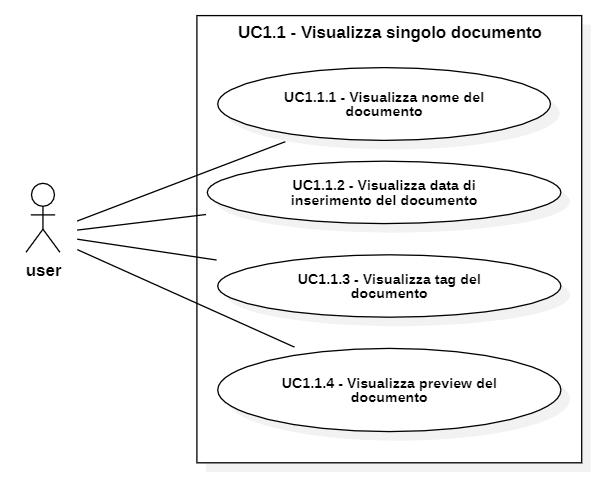
\includegraphics[width=0.8\linewidth]{UC1.1.1-2-3-4.png} %da modificare
    \caption{Diagramma UML dei casi d'uso UC-1.1.1, UC-1.1.2, UC-1.1.3 e UC-1.1.4} 
    \label{fig:UC3.1.1-2-3-4}
\end{figure}

\subsection{UC-2 Ricerca documento}
\begin{description}
    \item[Descrizione:] L’utente vuole poter ricercare un documento per nome, tag e/o data di inserimento.
    \item[Attore primario:] Utente generico.
    \item[Pre condizioni:] Il sistema mostra l’intera lista di documenti.
    \item[Post condizioni:] Il sistema mostra la lista di documenti che soddisfano la ricerca.
    \item[Scenario:]
    \begin{enumerate}
        \item[]
        \item L’utente seleziona la barra di ricerca per cercare un documento.
    \end{enumerate}
\end{description}

\begin{figure}[H]
    \centering
    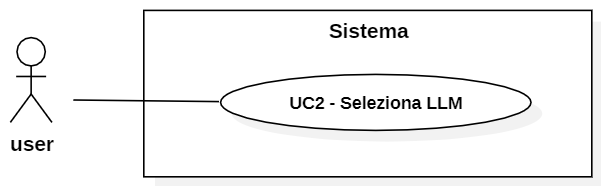
\includegraphics[width=0.8\linewidth]{UC2.PNG} %da modificare
    \caption{Diagramma UML del caso d'uso UC-2}
    \label{fig:UC4}
\end{figure}

\subsection{UC-2.1 Ricerca documento per nome}
\begin{description}
    \item[Descrizione:] L’utente vuole poter ricercare un documento per nome.
    \item[Attore primario:] Utente generico.
    \item[Pre condizioni:] Il sistema mostra l’intera lista di documenti.
    \item[Post condizioni:] Il sistema mostra la lista di documenti che contengono il nome inserito.
    \item[Scenario:] 
    \begin{enumerate}
        \item[]
        \item L’utente seleziona la barra di ricerca per cercare un documento (\textbf{UC-2}).
        \item L’utente inserisce il nome del file da cercare.
    \end{enumerate}
\end{description}

\subsection{UC-2.2 Ricerca documento per data}
\begin{description}
    \item[Descrizione:] L’utente vuole poter ricercare un documento per data di inserimento.
    \item[Attore primario:] Utente generico.
    \item[Pre condizioni:] Il sistema mostra l’intera lista di documenti.
    \item[Post condizioni:] Il sistema mostra la lista di documenti che sono stati inseriti dopo una certa data.
    \item[Scenario:] 
    \begin{enumerate}
        \item[]
        \item L’utente seleziona la barra di ricerca per cercare un documento (\textbf{UC-2}).
        \item L’utente inserisce la data di caricamento da cercare.
    \end{enumerate}
\end{description}

\subsection{UC-2.3 Ricerca documento per tag}
\begin{description}
    \item[Descrizione:] L’utente vuole poter ricercare un documento per il proprio tag.
    \item[Attore primario:] Utente generico.
    \item[Pre condizioni:] Il sistema mostra l’intera lista di documenti.
    \item[Post condizioni:] Il sistema mostra la lista di documenti che hanno quel tag.
    \item[Scenario:] 
    \begin{enumerate}
        \item[]
        \item L’utente seleziona la barra di ricerca per cercare un documento (\textbf{UC-2}).
        \item L’utente inserisce il tag da cercare.
    \end{enumerate}
\end{description}

\begin{figure}[H]
    \centering
    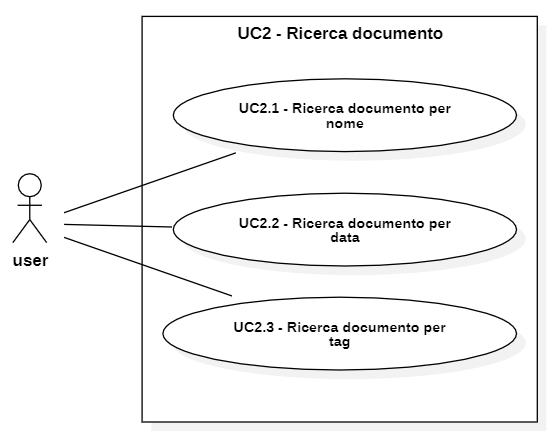
\includegraphics[width=0.8\linewidth]{UC2.1-2-3.png} %da modificare
    \caption{Diagramma UML dei casi d'uso UC-2.1, UC-2.2 e UC-2.3}
    \label{fig:UC4.1-2-3}
\end{figure}

\subsection{UC-3 Aggiungi tag al documento}
\begin{description}
    \item[Descrizione:] L’utente vuole poter aggiungere un tag ad un documento.
    \item[Attore primario:] Utente generico.
    \item[Pre condizioni:] Il documento non ha il tag voluto dall’utente.
    \item[Post condizioni:] Il documento ha il nuovo tag selezionato dall’utente.
    \item[Scenario:]
    \begin{enumerate}
        \item[]
        \item L’utente visualizza la lista di tutti documenti (\textbf{UC-1}).
        \item L'utente seleziona il documento.
        \item L’utente visualizza la lista di tag possibili.
        \item L’utente seleziona il tag da aggiungere.
    \end{enumerate}
\end{description}

\begin{figure}[H]
    \centering
    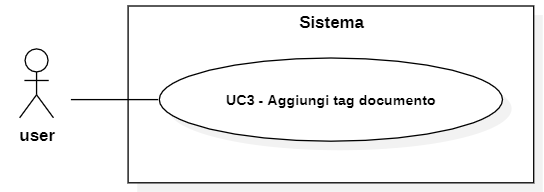
\includegraphics[width=0.8\linewidth]{UC3.png} %da modificare
    \caption{Diagramma UML del caso d'uso UC-3}
    \label{fig:UC5}
\end{figure}

\subsection{UC-4 Rimuovi tag dal documento}
\begin{description}
    \item[Descrizione:] L’utente vuole poter rimuovere un tag da un documento.
    \item[Attore primario:] Utente generico.
    \item[Pre condizioni:] Il documento ha associato il tag non più voluto dall’utente.
    \item[Post condizioni:] Il documento non ha più associato il tag non voluto dall’utente.
    \item[Scenario:]
    \begin{enumerate}
        \item[]
        \item L’utente visualizza la lista di tutti documenti (\textbf{UC-1}).
        \item L'utente seleziona il documento.
        \item L’utente visualizza la lista di tag associati a quel documento.
        \item L’utente seleziona il tag da rimuovere.
    \end{enumerate}
\end{description}

\begin{figure}[H]
    \centering
    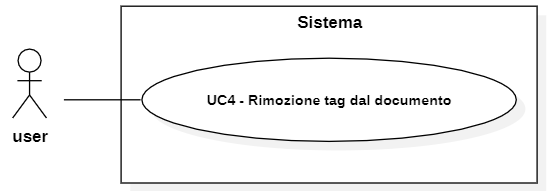
\includegraphics[width=0.8\linewidth]{UC4.png} %da modificare
    \caption{Diagramma UML del caso d'uso UC-4}
    \label{fig:UC6}
\end{figure}

\subsection{UC-5 Creazione nuovo tag}
\begin{description}
    \item[Descrizione:] L’utente vuole poter creare un tag da poter associare ad un documento.
    \item[Attore primario:] Utente generico.
    \item[Pre condizioni:] Il sistema non presenta il nuovo tag voluto dall’utente.
    \item[Post condizioni:] Il sistema presenta il tag voluto dall’utente.
    \item[Scenario:]
    \begin{enumerate}
        \item[]
        \item L’utente visualizza la lista di tutti i tag (\textbf{UC-6}).
        \item L'utente aggiunge un tag alla lista.
    \end{enumerate}
\end{description}

\begin{figure}[H]
    \centering
    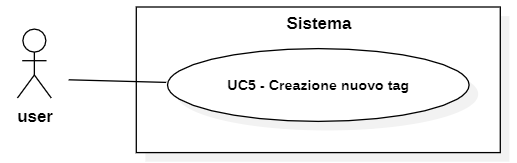
\includegraphics[width=0.8\linewidth]{UC5.png} %da modificare
    \caption{Diagramma UML del caso d'uso UC-5}
    \label{fig:UC7}
\end{figure}

\subsection{UC-5.1 Aggiungi nome del tag}
\begin{description}
    \item[Descrizione:] L’utente vuole poter aggiungere un nome nella creazione del tag.
    \item[Attore primario:] Utente generico.
    \item[Pre condizioni:] Il sistema non conosce il nome  il tag voluto dall’utente e il nome associato.
    \item[Post condizioni:] Il sistema conosce il nome del tag voluto dall’utente.
    \item[Scenario:]
    \begin{enumerate}
        \item[]
        \item L’utente visualizza la lista di tutti i tag (\textbf{UC-6}).
        \item L'utente aggiunge un tag alla lista (\textbf{UC-5}).
        \item L'utente inserisce il nome del nuovo tag.
    \end{enumerate}
\end{description}

\subsection{UC-5.2 Aggiungi colore del tag}
\begin{description}
    \item[Descrizione:] L’utente vuole poter aggiungere un colore nella creazione del tag.
    \item[Attore primario:] Utente generico.
    \item[Pre condizioni:] Il sistema non conosce il colore il tag voluto dall’utente.
    \item[Post condizioni:] Il sistema conosce il tag voluto dall’utente.
    \item[Scenario:]
    \begin{enumerate}
        \item[]
        \item L’utente visualizza la lista di tutti i tag (\textbf{UC-6}).
        \item L'utente aggiunge un tag alla lista (\textbf{UC-5}).
        \item L'utente inserisce il colore del nuovo tag.
    \end{enumerate}
\end{description}

\subsection{UC-5.3 Aggiungi descrizione del tag}
\begin{description}
    \item[Descrizione:] L’utente vuole poter aggiungere una descrizione opzionale nella creazione del tag.
    \item[Attore primario:] Utente generico.
    \item[Pre condizioni:] Il sistema non conosce la descrizione  del tag voluto dall’utente.
    \item[Post condizioni:] Il sistema conosce la descrizione del tag voluto dall’utente.
    \item[Scenario:]
    \begin{enumerate}
        \item[]
        \item L’utente visualizza la lista di tutti i tag (\textbf{UC-6}).
        \item L'utente aggiunge un tag alla lista (\textbf{UC-5}).
        \item L'utente inserisce la descrizione del nuovo tag.
    \end{enumerate}
\end{description}
\begin{figure}[H]
    \centering
    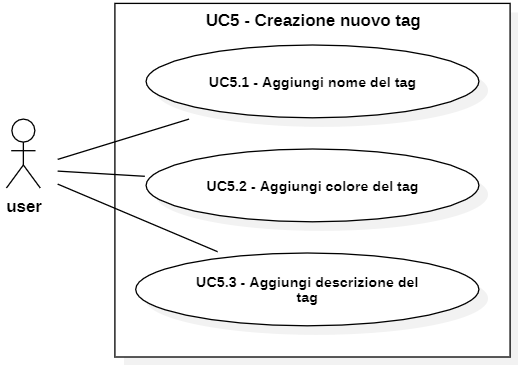
\includegraphics[width=0.8\linewidth]{UC5.1-2-3.png} %da modificare
    \caption{Diagramma UML dei casi d'uso UC-5.1, UC-5.2 e UC-5.3}
    \label{fig:UC7.1-2-3}
\end{figure}

\subsection{UC-6 Visualizza lista tag}
\begin{description}
    \item[Descrizione:] L’utente vuole poter visualizzare la lista di tutti i tag creati.
    \item[Attore primario:] Utente generico.
    \item[Pre condizioni:] Il sistema mostra l'interfaccia di gestione dei documenti.
    \item[Post condizioni:] Il sistema mostra la lista dei tag creati.
    \item[Scenario:]
    \begin{enumerate}
        \item[]
        \item L’utente visualizza la lista di tutti i tag.
    \end{enumerate}
\end{description}
\begin{figure}[H]
    \centering
    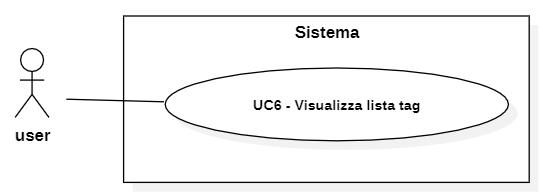
\includegraphics[width=0.8\linewidth]{UC6.png} %da modificare
    \caption{Diagramma UML del caso d'uso UC-6}
    \label{fig:UC8}
\end{figure}

\subsection{UC-6.1 Visualizza singolo tag}
\begin{description}
    \item[Descrizione:] L’utente vuole poter visualizzare uno dei tag creati.
    \item[Attore primario:] Utente generico.
    \item[Pre condizioni:] Il sistema mostra la lista dei tag creati.
    \item[Post condizioni:] Il sistema mostra il tag di interesse.
    \item[Scenario:]
    \begin{enumerate}
        \item[]
        \item L’utente visualizza la lista di tutti i tag (\textbf{UC-6}).
        \item L'utente visualizza un singolo tag.
    \end{enumerate}
\end{description}

\begin{figure}[H]
    \centering
    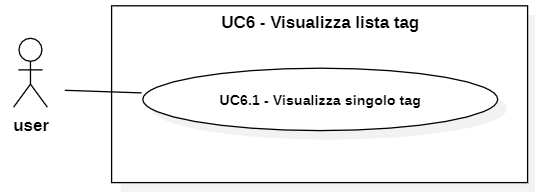
\includegraphics[width=0.8\linewidth]{UC6.1.png} %da modificare
    \caption{Diagramma UML del caso d'uso UC-6.1}
    \label{fig:UC8.10}
\end{figure}
\subsection{UC-6.1.1 Visualizza nome del tag}
\begin{description}
    \item[Descrizione:] L’utente vuole poter visualizzare il nome del tag di interesse.
    \item[Attore primario:] Utente generico.
    \item[Pre condizioni:] Il sistema mostra la lista dei tag creati.
    \item[Post condizioni:] Il sistema mostra il nome del tag selezionato.
    \item[Scenario:]
    \begin{enumerate}
        \item[]
        \item L’utente visualizza la lista di tutti i tag (\textbf{UC-6}).
        \item L'utente visualizza un singolo tag (\textbf{UC-6.1}).
        \item L'utente visualizza il nome del tag.
    \end{enumerate}
\end{description}

\subsection{UC-6.1.2 Visualizza colore del tag}
\begin{description}
    \item[Descrizione:] L’utente vuole poter visualizzare il colore del tag di interesse.
    \item[Attore primario:] Utente generico.
    \item[Pre condizioni:] Il sistema mostra la lista dei tag creati.
    \item[Post condizioni:] Il sistema mostra il colore del tag selezionato.
    \item[Scenario:] 
    \begin{enumerate}
        \item[]
        \item L’utente visualizza la lista di tutti i tag (\textbf{UC-6}).
        \item L'utente visualizza un singolo tag (\textbf{UC-6.1}).
        \item L'utente visualizza il colore del tag.
    \end{enumerate}
\end{description}

\subsection{UC-6.1.3 Visualizza descrizione del tag}
\begin{description}
    \item[Descrizione:] L’utente vuole poter visualizzare la descrizione del tag di interesse.
    \item[Attore primario:] Utente generico.
    \item[Pre condizioni:] Il sistema mostra la lista dei tag creati.
    \item[Post condizioni:] Il sistema mostra la descrizione del tag selezionato.
    \item[Scenario:]
    \begin{enumerate}
        \item[]
        \item L’utente visualizza la lista di tutti i tag (\textbf{UC-6}).
        \item L'utente visualizza un singolo tag (\textbf{UC-6.1}).
        \item L'utente visualizza la descrizione del tag.
    \end{enumerate}
\end{description}

\begin{figure}[H]
    \centering
    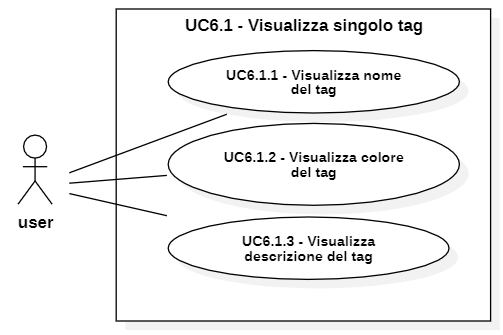
\includegraphics[width=0.8\linewidth]{UC6.1.1-2-3.png} %da modificare
    \caption{Diagramma UML dei casi d'uso UC-6.1.1, UC-6.1.2 e UC-6.1.3}
    \label{fig:UC8.1.1-2-3}
\end{figure}

\subsection{UC-7 Elimina tag}
\begin{description}
    \item[Descrizione:] L'utente vuole eliminare uno dei tag presenti nel sistema.
    \item[Attore primario:] Utente generico.
    \item[Pre condizioni:] Il sistema presenta il tag non desiderato.
    \item[Post condizioni:] Il sistema non presenta più il tag indesiderato.
    \item[Scenario:]
    \begin{enumerate}
        \item[]
        \item L’utente visualizza la lista di tutti i tag (\textbf{UC-6}).
        \item L'utente visualizza un singolo tag (\textbf{UC-6.1}).
        \item L'utente elimina il tag visualizzato.
    \end{enumerate}
\end{description}

\begin{figure}[H]
    \centering
    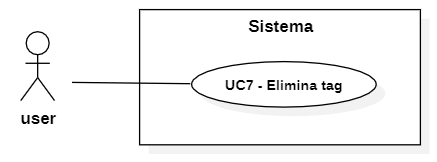
\includegraphics[width=0.8\linewidth]{UC7.png} %da modificare
    \caption{Diagramma UML del caso d'uso UC-7}
    \label{fig:UC9}
\end{figure}

\subsection{UC-8 Elimina documento}
\begin{description}
    \item[Descrizione:] L'utente vuole eliminare uno dei documenti presenti nel sistema.
    \item[Attore primario:] Utente generico.
    \item[Pre condizioni:] Il sistema presenta il documento non desiderato.
    \item[Post condizioni:] Il sistema non presenta più il documento indesiderato.
    \item[Scenario:]
    \begin{enumerate}
        \item[]
        \item L’utente visualizza la lista di tutti documenti (\textbf{UC-1}).
        \item L'utente visualizza il singolo documento (\textbf{UC-1.1}).
        \item L'utente elimina il documento d'interesse.
    \end{enumerate} 
\end{description}

\subsection{UC-8.1 Conferma eliminazione documento}
\begin{description}
    \item[Descrizione:] L'utente vuole confermare l'eliminazione di uno dei documenti presenti nel sistema.
    \item[Attore primario:] Utente generico.
    \item[Pre condizioni:] Il sistema presenta il documento non desiderato.
    \item[Post condizioni:] Il sistema non presenta più il documento indesiderato.
    \item[Scenario:] 
    \begin{enumerate}
        \item[]
        \item L’utente visualizza la lista di tutti documenti (\textbf{UC-1}).
        \item L'utente visualizza il singolo documento (\textbf{UC-1.1}).
        \item L'utente elimina il documento d'interesse (\textbf{UC-8}).
        \item L'utente conferma l'eliminazione del documento dal sistema.
    \end{enumerate}
    
\end{description}

\begin{figure}[H]
    \centering
    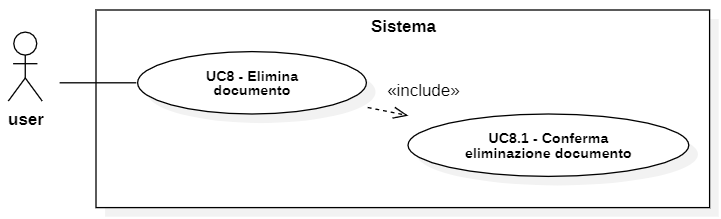
\includegraphics[width=0.8\linewidth]{UC8.png} %da modificare
    \caption{Diagramma UML dei casi d'uso UC-8, UC-8.1}
    \label{fig:UC10-11}
\end{figure}

\subsection{UC-9 Aggiungi documento}
\begin{description}
    \item[Descrizione:] L'utente vuole aggiungere un documento nel sistema.
    \item[Attore primario:] Utente generico.
    \item[Pre condizioni:] Il sistema non presenta il documento di interesse.
    \item[Post condizioni:] Nel sistema è presente un nuovo documento.
    \item[Scenario:]
    \begin{enumerate}
        \item[]
        \item L’utente aggiunge un nuovo documento.
    \end{enumerate}
    \item[Generalizzazioni:] 
    \begin{itemize}
        \item[] 
        \item Aggiungi documento tramite trascinamento (\textbf{UC-9.1});
        \item Aggiungi documento tramite file system (\textbf{UC-9.2}).
    \end{itemize} 
    \item[Scenario alternativo:] Visualizza errore nell'inserimento di un documento (\textbf{UC-10}).
\end{description}

\subsection{UC-9.1 Aggiungi documento tramite trascinamento}
\begin{description}
    \item[Descrizione:] L'utente vuole aggiungere un documento nel sistema tramite trascinamento.
    \item[Attore primario:] Utente generico.
    \item[Pre condizioni:] Il sistema non presenta il documento di interesse.
    \item[Post condizioni:] Nel sistema è presente un nuovo documento.
    \item[Scenario:] 
    \begin{enumerate}
        \item[]
        \item L’utente aggiunge un nuovo documento (\textbf{UC-10}).
        \item L'utente aggiunge un nuovo documento nel sistema tramite trascinamento.
    \end{enumerate}
\end{description}

\subsection{UC-9.2 Aggiungi documento tramite file system}
\begin{description}
    \item[Descrizione:] L'utente vuole aggiungere un documento nel sistema tramite navigazione del file system.
    \item[Attore primario:] Utente generico.
    \item[Pre condizioni:] Il sistema non presenta il documento di interesse.
    \item[Post condizioni:] Nel sistema è presente un nuovo documento.
    \item[Scenario:]
    \begin{enumerate}
        \item[]
        \item L’utente aggiunge un nuovo documento (\textbf{UC-10}).
        \item L'utente aggiunge un nuovo documento nel sistema tramite navigazione del file system.
    \end{enumerate}
\end{description}

\subsection{UC-10 Visualizza errore inserimento documento}
\begin{description}
    \item[Descrizione:] L'utente visualizza un messaggio che lo notifica che c'è stato un errore nell'inserimento del documento.
    \item[Attore primario:] Utente generico.
    \item[Pre condizioni:] L'utente tenta di inserire un documento nel sistema.
    \item[Post condizioni:] Il sistema notifica un messaggio di errore e il documento non viene inserito nel sistema.
    \item[Scenario:]
    \begin{enumerate}
        \item[]
        \item L’utente aggiunge un nuovo documento (\textbf{UC-9}).
        \item L'utente visualizza un messaggio d'errore.
    \end{enumerate}
    \item[Generalizzazioni:]
    \begin{itemize}
        \item[] 
        \item Visualizza errore nome file già presente (\textbf{UC-10.1});
        \item Visualizza errore formato file (\textbf{UC-10.2});
        \item Visualizza errore file corrotto (\textbf{UC-10.3}).
    \end{itemize}
\end{description}

\subsection{UC-10.1 Visualizza errore nome file già presente}
\begin{description}
    \item[Descrizione:] L'utente visualizza un messaggio che lo notifica che c'è stato un errore nell'inserimento del documento dovuto al nome del file già in uso.
    \item[Attore primario:] Utente generico.
    \item[Pre condizioni:] L'utente tenta di inserire nel sistema un documento con un nome già in uso.
    \item[Post condizioni:] Il sistema notifica un messaggio di errore e il documento non viene inserito nel sistema.
    \item[Scenario:]
    \begin{enumerate}
        \item[]
        \item L’utente aggiunge un nuovo documento (\textbf{UC-9}).
        \item L'utente visualizza un messaggio d'errore (\textbf{UC-10}).
        \item L'utente visualizza un messaggio d'errore a seguito di un tentativo di aggiungere un nuovo documento a sistema con un nome già in uso.
    \end{enumerate}
\end{description}

\subsection{UC-10.2 Visualizza errore formato file}
\begin{description}
    \item[Descrizione:] L'utente visualizza un messaggio che lo notifica che c'è stato un errore nell'inserimento del documento dovuto al formato del file non supportato.
    \item[Attore primario:] Utente generico.
    \item[Pre condizioni:] L'utente tenta di inserire nel sistema un documento con un formato non supportato.
    \item[Post condizioni:] Il sistema notifica un messaggio di errore e il documento non viene inserito nel sistema.
    \item[Scenario:] 
    \begin{enumerate}
        \item[]
        \item L’utente aggiunge un nuovo documento (\textbf{UC-9}).
        \item L'utente visualizza un messaggio d'errore (\textbf{UC-10}).
        \item L'utente visualizza un messaggio di errore, a seguito di un tentativo di aggiungere un nuovo documento a sistema con un formato non supportato.
    \end{enumerate}
\end{description}

\subsection{UC-10.3 Visualizza errore file corrotto}
\begin{description}
    \item[Descrizione:] L'utente visualizza un messaggio che lo notifica che c'è stato un errore nell'inserimento del documento dovuto alla corruzione del file.
    \item[Attore primario:] Utente generico.
    \item[Pre condizioni:] L'utente tenta di inserire nel sistema un documento corrotto.
    \item[Post condizioni:] Il sistema notifica un messaggio di errore e il documento non viene inserito nel sistema.
    \item[Scenario:]
    \begin{enumerate}
        \item[]
        \item L’utente aggiunge un nuovo documento (\textbf{UC-9}).
        \item L'utente visualizza un messaggio d'errore (\textbf{UC-10}).
        \item L'utente visualizza un messaggio di errore, a seguito di un tentativo di aggiungere un nuovo documento a sistema tramite un file corrotto.
    \end{enumerate}
\end{description}

\begin{figure}[H]
    \centering
    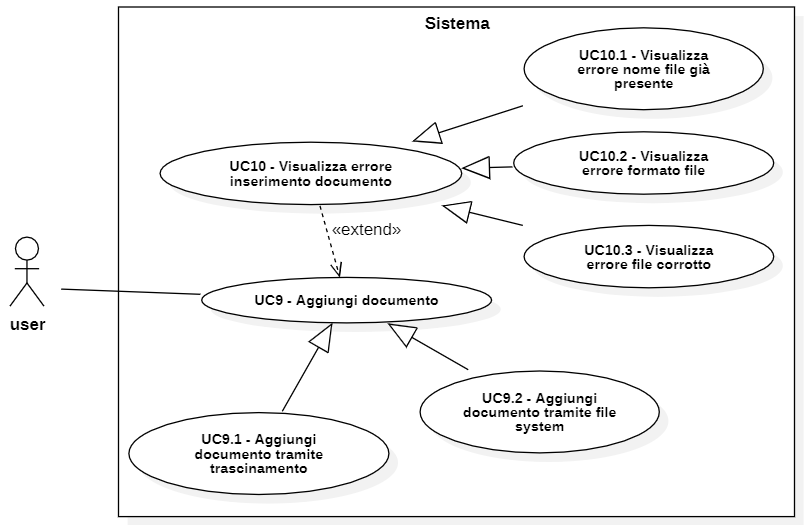
\includegraphics[width=\linewidth]{UC9-10.png} %da modificare
    \caption{Diagramma UML dei casi d'uso UC-9, UC-9.1, UC-9.2, UC-10, UC-10.1, UC-10.2 e UC-10.3}
    \label{fig:UC12-13}
\end{figure}

\subsection{UC-11 Visualizza lista lingue chatbot}
\begin{description}
    \item[Descrizione:] L'utente vuole visualizzare la lista delle lingue supportate dal chatbot.
    \item[Attore primario:] Utente generico.
    \item[Pre condizioni:] Il sistema mostra l'interfaccia del chatbot.
    \item[Post condizioni:] Il sistema mostra la lista delle lingue supportate.
    \item[Scenario:]
    \begin{enumerate}
        \item[]
        \item L'utente visualizza la lista delle lingue supportate
    \end{enumerate}
\end{description}

\begin{figure}[H]
    \centering
    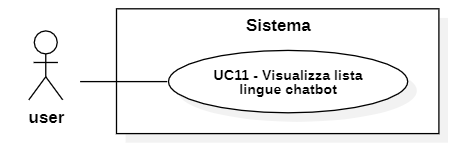
\includegraphics[width=0.8\linewidth]{UC11.png} %da modificare
    \caption{Diagramma UML del caso d'uso UC-11}
    \label{fig:UC14}
\end{figure}

\subsection{UC-12 Seleziona lingua del chatbot}
\begin{description}
    \item[Descrizione:] L'utente vuole selezionare la lingua del sistema.
    \item[Attore primario:] Utente generico.
    \item[Pre condizioni:] Il sistema mostra la lista delle lingue supportate.
    \item[Post condizioni:] Il sistema aggiorna la lingua del chatbot.
    \item[Scenario:]
    \begin{enumerate}
        \item[]
        \item L'utente visualizza la lista delle lingue supportate (\textbf{UC-12})
        \item L’utente seleziona la lingua del chatbot tra quelle supportate.
    \end{enumerate}
\end{description}

\begin{figure}[H]
    \centering
    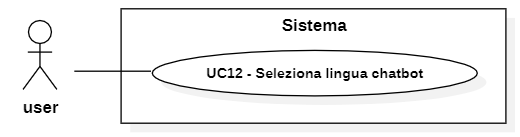
\includegraphics[width=0.8\linewidth]{UC12.png} %da modificare
    \caption{Diagramma UML del caso d'uso UC-12}
    \label{fig:UC15}
\end{figure}

\subsection{UC-13 Inserisci domanda}
\begin{description}
    \item[Descrizione:] L'utente vuole inserire una domanda per il chatbot.
    \item[Attore primario:] Utente generico.
    \item[Pre condizioni:] Il sistema mostra l'interfaccia del chatbot.
    \item[Post condizioni:] Il sistema presenta la domanda dell'utente nello spazio relativo.
    \item[Scenario:]
    \begin{enumerate}
        \item[]
        \item L’utente pone una domanda al chatbot.
    \end{enumerate}
    \item[Generalizzazioni:] 
    \begin{itemize}
        \item[] 
        \item Digita domanda (\textbf{UC-13.1});
        \item Input vocale della domanda (\textbf{UC-13.2}) .
    \end{itemize}
\end{description}

\subsection{UC-13.1 Digita domanda}
\begin{description}
    \item[Descrizione:] L'utente vuole digitare la domanda da porgere al chatbot.
    \item[Attore primario:] Utente generico.
    \item[Pre condizioni:] Il sistema mostra l'interfaccia del chatbot.
    \item[Post condizioni:] Il sistema presenta la domanda digitata dall'utente nello spazio relativo.
    \item[Scenario:]
    \begin{enumerate}
        \item[]
        \item L’utente pone una domanda al chatbot (\textbf{UC-13}).
        \item L'utente inserisce la domanda da rivolgere al sistema digitandola.
    \end{enumerate}
\end{description}

\subsection{UC-13.2 Input vocale della domanda}
\begin{description}
    \item[Descrizione:] L'utente vuole inserire tramite microfono la domanda da porgere al sistema.
    \item[Attore primario:] Utente generico.
    \item[Pre condizioni:] Il sistema mostra l'interfaccia del chatbot.
    \item[Post condizioni:] Il sistema presenta la domanda posta a voce dall'utente nello spazio relativo.
    \item[Scenario:]
    \begin{enumerate}
        \item[]
        \item L’utente pone una domanda al chatbot (\textbf{UC-14}).
        \item L'utente inserisce la domanda da rivolgere al chatbot tramite input vocale.
    \end{enumerate}
    \item[Scenario alternativo:] Visualizza errore nell'inserimento della domanda tramite input vocale (\textbf{UC-14}).
\end{description}

\subsection{UC-14 Visualizza errore input vocale}
\begin{description}
    \item[Descrizione:] L'utente ha tentato di inserire senza successo la domanda da porre al sistema tramite input vocale.
    \item[Attore primario:] Utente generico.
    \item[Pre condizioni:] L'utente tenta di inserire la domanda tramite input vocale.
    \item[Post condizioni:] Il sistema non presenta la domanda posta a voce dall'utente nello spazio relativo.
    \item[Scenario:] 
    \begin{enumerate}
        \item[]
        \item L’utente pone una domanda al chatbot (\textbf{UC-13}).
        \item L'utente inserisce la domanda da rivolgere al chatbot tramite input vocale (\textbf{UC-13.2}).
        \item L'utente visualizza un messaggio di errore, a seguito di un tentativo fallito di inserire tramite input vocale la domanda da porre al sistema.
    \end{enumerate}
\end{description}

\begin{figure}[H]
    \centering
    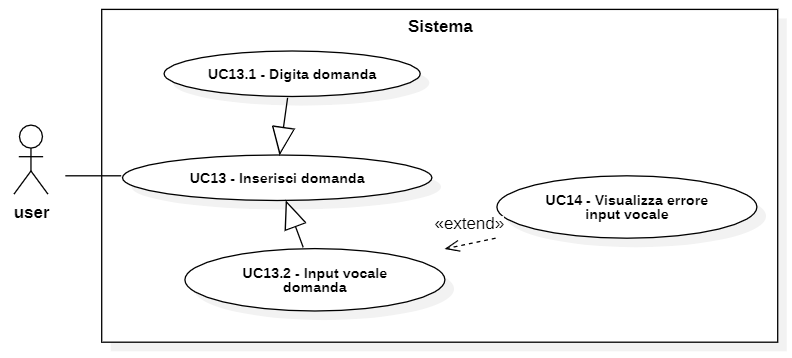
\includegraphics[width=\linewidth]{UC13-14.png} %da modificare
    \caption{Diagramma UML dei casi d'uso UC-13, UC-13.1, UC-13.2 e UC-14}
    \label{fig:UC16-17}
\end{figure}

\subsection{UC-15 Invia domanda}
\begin{description}
    \item[Descrizione:] L'utente vuole inviare una domanda al sistema.
    \item[Attore primario:] Utente generico.
    \item[Pre condizioni:] Il sistema presenta la domanda posta dall'utente.
    \item[Post condizioni:] Il sistema ha processato correttamente la domanda inserita dall'utente.
    \item[Scenario:]
    \begin{enumerate}
        \item[]
        \item L’utente pone una domanda al chatbot (\textbf{UC-13}).
        \item L'utente invia la domanda al sistema.
    \end{enumerate}
    \item[Scenario alternativo:] Visualizza errore invio domanda (\textbf{UC-16}).
\end{description}

\subsection{UC-16 Visualizza errore invio domanda}
\begin{description}
    \item[Descrizione:] L'utente visualizza un messaggio che lo informa che c'è stato un errore nell'invio della domanda.
    \item[Attore primario:] Utente generico.
    \item[Pre condizioni:] L'utente ha tentato di inviare una domanda.
    \item[Post condizioni:] Il sistema notifica un messaggio di errore e non invia la domanda.
    \item[Scenario:] 
    \begin{enumerate}
        \item[]
        \item L’utente pone una domanda al chatbot (\textbf{UC-13}).
        \item L'utente invia la domanda al sistema (\textbf{UC-15}).
        \item L'utente visualizza un messaggio di errore, a seguito di un tentativo di inviare una domanda.
    \end{enumerate}
\end{description}

\begin{figure}[H]
    \centering
    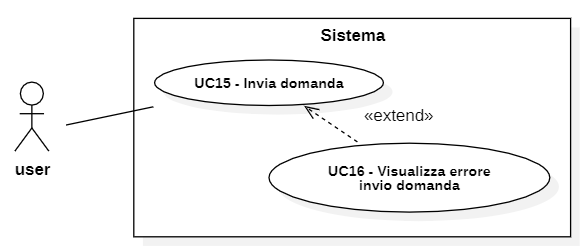
\includegraphics[width=\linewidth]{UC15-16.png} %da modificare
    \caption{Diagramma UML dei casi d'uso UC-15 e UC-16}
    \label{fig:UC18-19}
\end{figure}

\subsection{UC-17 Visualizza risposta}
\begin{description}
    \item[Descrizione:] L'utente vuole visualizzare la risposta alla domanda che ha inviato in precedenza.
    \item[Attore primario:] Utente generico.
    \item[Attore secondario:] Modello LLM. 
    \item[Pre condizioni:] Il sistema ha ricevuto e processato la domanda posta dall'utente.
    \item[Post condizioni:] Il sistema restituisce una risposta all'utente.
    \item[Scenario:]
    \begin{enumerate}
        \item[]
        \item L’utente pone una domanda al chatbot (\textbf{UC-13}).
        \item L'utente invia la domanda al sistema (\textbf{UC-15}).
        \item L'utente visualizza la risposta alla domanda posta al sistema.
    \end{enumerate}
    \item[Generalizzazioni:]
    \begin{itemize}
        \item[] 
        \item Visualizza risposta alla domanda (\textbf{UC-17.1});
        \item Visualizza risposta di cortesia (\textbf{UC-17.2}).
    \end{itemize}
    \item[Scenario alternativo:] Visualizza un errore risposta (\textbf{UC-18}).
\end{description}

\subsection{UC-17.1 Visualizza risposta domanda}
\begin{description}
    \item[Descrizione:] L'utente vuole visualizzare la risposta alla domanda che ha inviato in precedenza.
    \item[Attore primario:] Utente generico.
    \item[Attore secondario:] Modello LLM. 
    \item[Pre condizioni:] Il sistema ha ricevuto e processato la domanda posta dall'utente.
    \item[Post condizioni:] Il sistema restituisce una risposta della domanda all'utente.
    \item[Scenario:]
    \begin{enumerate}
        \item[]
        \item L’utente pone una domanda pertinente al documento al chatbot (\textbf{UC-13}).
        \item L'utente invia la domanda al sistema (\textbf{UC-15}).
        \item L'utente visualizza la risposta alla domanda posta al sistema.
    \end{enumerate}
    \item[Scenario alternativo:] Visualizza un errore risposta (\textbf{UC-18}).
\end{description}

\subsection{UC-17.2 Visualizza risposta di cortesia}
\begin{description}
    \item[Descrizione:] L'utente vuole visualizzare la risposta alla domanda che ha inviato in precedenza.
    \item[Attore primario:] Utente generico.
    \item[Attore secondario:] Modello LLM. 
    \item[Pre condizioni:] Il sistema ha ricevuto e processato la domanda posta dall'utente.
    \item[Post condizioni:] Il sistema restituisce una risposta di cortesia all'utente.
    \item[Scenario:]
    \begin{enumerate}
        \item[]
        \item L’utente pone una domanda non pertinente al documento al chatbot (\textbf{UC-13}).
        \item L'utente invia la domanda al sistema (\textbf{UC-15}).
        \item L'utente visualizza la risposta alla domanda posta al sistema.
    \end{enumerate}
    \item[Scenario alternativo:] Visualizza un errore risposta (\textbf{UC-18}).
\end{description}

\subsection{UC-18 Visualizza errore risposta}
\begin{description}
    \item[Descrizione:] L'utente visualizza un messaggio che lo informa che c'è stato un errore nel ricevere la risposta.
    \item[Attore primario:] Utente generico.
    \item[Pre condizioni:] 
    \item[Post condizioni:] Il sistema notifica un messaggio di errore e non restituisce la risposta.
    \item[Scenario:] 
    \begin{enumerate}
        \item[]
        \item L’utente pone una domanda al chatbot (\textbf{UC-13}).
        \item L'utente invia la domanda al sistema (\textbf{UC-15}).
        \item L'utente visualizza un errore nella visualizzazione della risposta.
    \end{enumerate}
\end{description}

\begin{figure}[H]
    \centering
    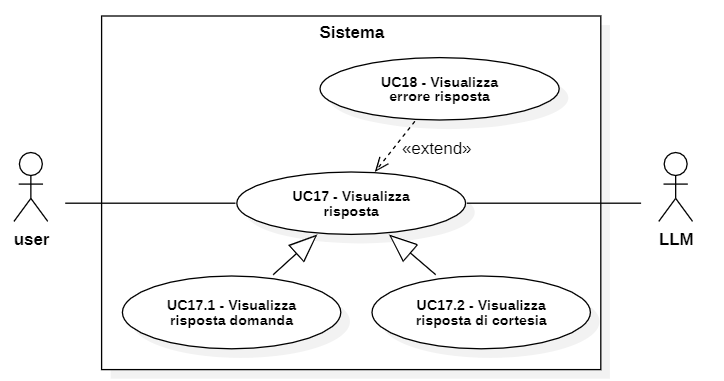
\includegraphics[width=0.8\linewidth]{UC17-18.png} %da modificare
    \caption{Diagramma UML dei casi d'uso UC-17, UC-17.1, UC-17-2 e UC-18}
    \label{fig:UC20-21}
\end{figure}

\subsection{UC-19 Crea nuova sessione}
\begin{description}
    \item[Descrizione:] L'utente vuole creare una nuova sessione di conversazione col chatbot.
    \item[Attore primario:] Utente generico.
    \item[Pre condizioni:] Il sistema non presenta la nuova sessione di interesse dell'utente.
    \item[Post condizioni:] Il sistema inizializza una nuova sessione.
    \item[Scenario:] 
    \begin{enumerate}
        \item[]
        \item L'utente crea una nuova sessione di conversazione nel sistema.
    \end{enumerate}
    \item[Scenario alternativo:] Visualizza errore creazione sessione (\textbf{UC-20})
\end{description}

\subsection{UC-20 Visualizza errore creazione sessione}
\begin{description}
    \item[Descrizione:] L'utente visualizza un messaggio che lo notifica che c'è stato un errore nella creazione di una nuova sessione.
    \item[Attore primario:] Utente generico.
    \item[Pre condizioni:] L'utente ha tentato di creare una nuova sessione.
    \item[Post condizioni:] Il sistema notifica un messaggio di errore e non crea una nuova sessione.
    \item[Scenario:] 
    \begin{enumerate}
        \item[]
        \item L'utente crea una nuova sessione di conversazione nel sistema (\textbf{UC-19}).
        \item L'utente visualizza un messaggio di errore e non viene creata una nuova sessione.
    \end{enumerate}
\end{description}

\begin{figure}[H]
    \centering
    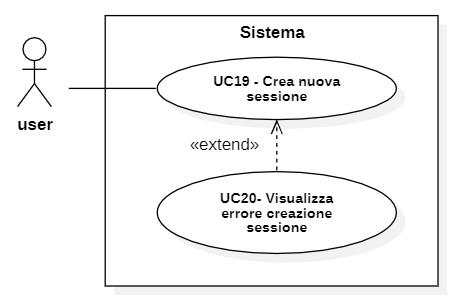
\includegraphics[width=0.8\linewidth]{UC19-20.png} %da modificare
    \caption{Diagramma UML dei casi d'uso UC-19 e UC-20}
    \label{fig:UC22-23}
\end{figure}

\subsection{UC-21 Visualizza lista sessioni aperte}
\begin{description}
    \item[Descrizione:] L'utente vuole visualizzare la lista delle sessioni di conversazione col chatbot aperte.
    \item[Attore primario:] Utente generico.
    \item[Pre condizioni:] Il sistema mostra l'interfaccia relativa al chatbot.
    \item[Post condizioni:] Il sistema mostra la lista delle sessioni attive.
    \item[Scenario:]
    \begin{enumerate}
        \item[]
        \item L'utente visualizza la lista delle sessioni attive.
    \end{enumerate}
    \item[Scenario alternativo:] Visualizza errore sessioni aperte (\textbf{UC-22})
\end{description}

\subsection{UC-21.1 Visualizza singola sessione}
\begin{description}
    \item[Descrizione:] L'utente vuole visualizzare una delle sessioni di conversazione col chatbot.
    \item[Attore primario:] Utente generico.
    \item[Pre condizioni:] Il sistema mostra la lista delle sessioni attive.
        \item[Post condizioni:] Il sistema mostra una particolare sessione attiva.
    \item[Scenario:] 
    \begin{enumerate}
        \item[]
        \item L'utente visualizza la lista delle sessioni attive (\textbf{UC-21}).
        \item L'utente visualizza una delle sessioni attive nel sistema.
    \end{enumerate}
\end{description}

\subsection{UC-22 Visualizza errore sessioni aperte }
\begin{description}
    \item[Descrizione:] L'utente visualizza un messaggio che lo notifica che c'è stato un errore nella visualizzazione delle sessioni aperte.
    \item[Attore primario:] Utente generico.
    \item[Pre condizioni:] Il sistema ha tentato di visualizzare le sessioni aperte.
    \item[Post condizioni:] Il sistema notifica un messaggio di errore e non visualizza le sessioni aperte.
    \item[Scenario:] 
    \begin{enumerate}
        \item[]
        \item L'utente visualizza la lista delle sessioni attive (\textbf{UC-21}).
        \item L'utente visualizza un messaggio di errore e non viene visualizzata la lista delle sessioni aperte.
    \end{enumerate}
\end{description}

\begin{figure}[H]
    \centering
    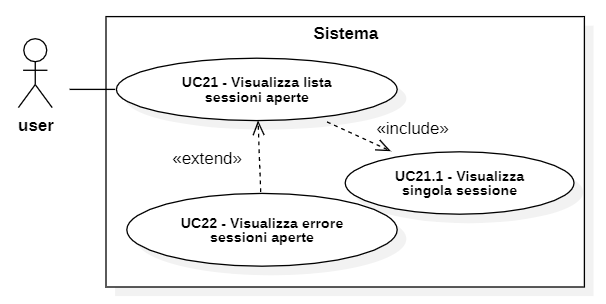
\includegraphics[width=0.8\linewidth]{UC21-22.png} %da modificare
    \caption{Diagramma UML dei casi d'uso UC-21, UC-21.1 e UC-22}
    \label{fig:UC24-25}
\end{figure}

\subsection{UC-23 Elimina sessione}
\begin{description}
    \item[Descrizione:] L'utente vuole eliminare una delle sessioni di conversazioni attive nel sistema.
    \item[Attore primario:] Utente generico.
    \item[Pre condizioni:] Il sistema presenta la sessione che l'utente vuole eliminare.
    \item[Post condizioni:] Il sistema non presenta più la sessione eliminata dall'utente.
    \item[Scenario:] 
    \begin{enumerate}
        \item[]
        \item L'utente visualizza la lista delle sessioni attive (\textbf{UC-21}).
        \item L'utente visualizza una delle sessioni attive nel sistema (\textbf{UC-21.1}).
        \item L'utente elimina dal sistema la sessione di conversazione con il chatbot desiderata.
    \end{enumerate}
\end{description}

\subsection{UC-23.1 Conferma eliminazione sessione}
\begin{description}
    \item[Descrizione:] L'utente vuole eliminare una delle sessioni di conversazioni attive nel sistema.
    \item[Attore primario:] Utente generico.
    \item[Pre condizioni:] Il sistema presenta la sessione che l'utente vuole eliminare.
    \item[Post condizioni:] Il sistema non presenta più la sessione eliminata dall'utente.
    \item[Scenario:] 
    \begin{enumerate}
        \item[]
        \item L'utente visualizza la lista delle sessioni attive (\textbf{UC-21}).
        \item L'utente visualizza una delle sessioni attive nel sistema (\textbf{UC-21.1}).
        \item L'utente elimina dal sistema la sessione di conversazione con il chatbot desiderata (\textbf{UC-23}).
        \item L'utente conferma l'eliminazione della sessione di conversazione dal sistema.
    \end{enumerate}
\end{description}

\begin{figure}[H]
    \centering
    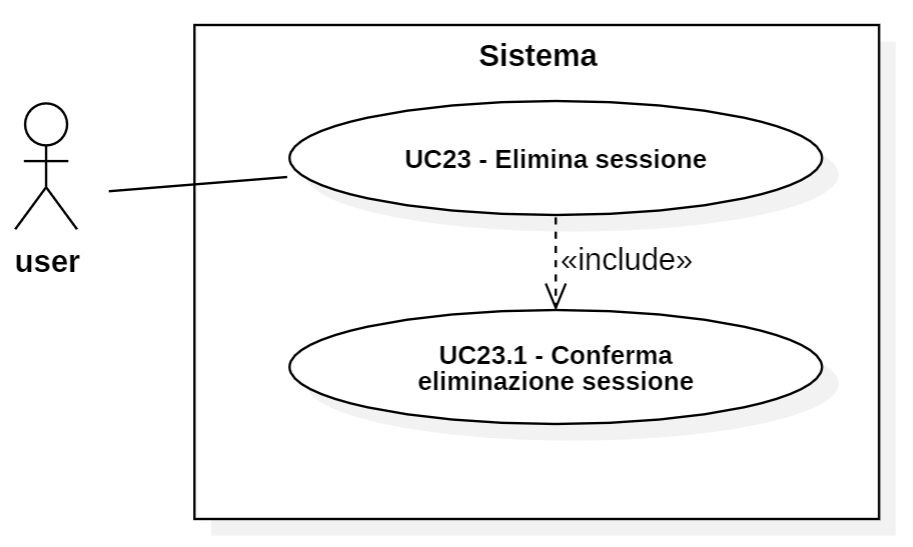
\includegraphics[width=0.9\linewidth]{UC23.png} %da modificare
    \caption{Diagramma UML dei casi d'uso UC-23 e UC-23.1}
    \label{fig:UC26-27}
\end{figure}

\subsection{UC-24 Visualizza chat history}
\begin{description}
    \item[Descrizione:] L'utente vuole visualizzare lo scambio di domande e risposte avvenuto in precedenza con il sistema in una sessione.
    \item[Attore primario:] Utente generico.
    \item[Pre condizioni:] Il sistema ha in precedenza ricevuto una o più domande a cui ha fornito risposte.
    \item[Post condizioni:] Il sistema mostra lo storico delle conversazioni dell'utente
    \item[Scenario:]
    \begin{enumerate}
        \item[]
        \item L'utente visualizza lo scambio di domande e risposte in una sessione con il sistema.
    \end{enumerate}
    
\end{description} 

\begin{figure}[H]
    \centering
    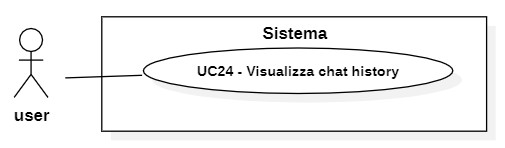
\includegraphics[width=0.9\linewidth]{UC24.png} %da modificare
    \caption{Diagramma UML dei casi d'uso UC-24}
    \label{fig:UC28-29}
\end{figure}

\subsection{UC-25 Elimina chat history}
\begin{description}
    \item[Descrizione:] L'utente vuole eliminare lo scambio di domande e risposte, avvenuto in precedenza con il chatbot, dalla sessione del sistema.
    \item[Attore primario:] Utente generico.
    \item[Pre condizioni:] Il sistema presenta la chat history.
    \item[Post condizioni:] Il sistema non presenta più alcuna chat history in quella sessione.
    \item[Scenario:]
    \begin{enumerate}
        \item[]
        \item L'utente elimina la chat history della sessione corrente.
    \end{enumerate}
\end{description}

\subsection{UC-25.1 Conferma eliminazione chat history}
\begin{description}
    \item[Descrizione:] L'utente vuole eliminare lo scambio di domande e risposte, avvenuto in precedenza con il chatbot, dalla sessione del sistema.
    \item[Attore primario:] Utente generico.
    \item[Pre condizioni:] Il sistema presenta la chat history.
    \item[Post condizioni:] Il sistema non presenta più alcuna chat history in quella sessione.
    \item[Scenario:]
    \begin{enumerate}
        \item[]
        \item L'utente elimina la chat history della sessione corrente (\textbf{UC-25}).
        \item L'utente conferma l'eliminazione della chat history della sessione corrente dal sistema.
    \end{enumerate}
\end{description}

\begin{figure}[H]
    \centering
    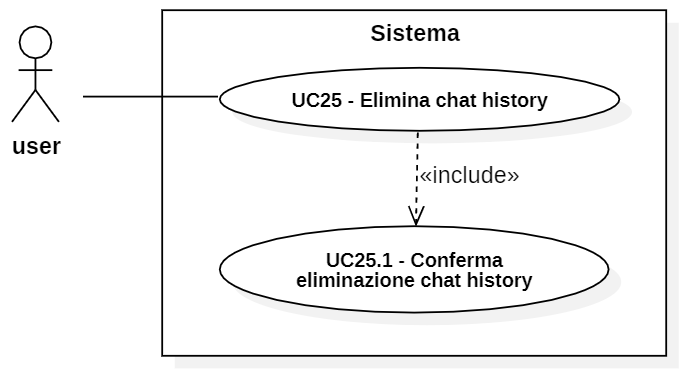
\includegraphics[width=0.9\linewidth]{UC25.png} %da modificare e aggiungere 25.1
    \caption{Diagramma UML dei casi d'uso UC-25 e 25.1}
    \label{fig:UC30-31}
\end{figure}

\subsection{UC-26 Visualizza informazioni risposta}
\begin{description}
    \item[Descrizione:] L'utente vuole visualizzare le informazioni del documento da cui deriva la risposta ricevuta.
    \item[Attore primario:] Utente generico.
    \item[Attore secondario:] Modello LLM.
    \item[Pre condizioni:] Il sistema mostra la risposta ad una domanda dell'utente.
    \item[Post condizioni:] Il sistema mostra le informazioni riguardanti la fonte della risposta.
    \item[Scenario:]
    \begin{enumerate}
        \item[]
        \item L’utente pone una domanda al chatbot (\textbf{UC-13}).
        \item L'utente invia la domanda al sistema (\textbf{UC-15}).
        \item L'utente visualizza la risposta alla domanda posta al sistema (\textbf{UC-17}).
        \item L'utente visualizza le informazioni sul documento fonte della risposta.
    \end{enumerate}
\end{description}

\begin{figure}[H]
    \centering
    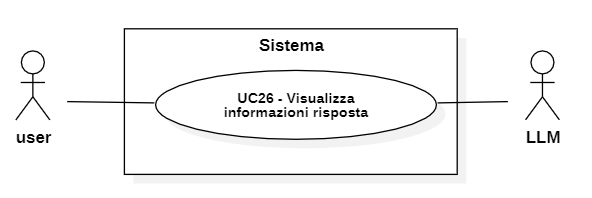
\includegraphics[width=0.9\linewidth]{UC26.png}  %da modificare E AGGIUNGERE ATTORE SECONDARIO LLM
    \caption{Diagramma UML del caso d'uso UC-26}
    \label{fig:UC32}
\end{figure}

\subsection{UC-26.1 Visualizza nome del documento}
\begin{description}
    \item[Descrizione:] L'utente vuole poter visualizzare il nome del documento relativo alla risposta.
    \item[Attore primario:] Utente generico.
    \item[Attore secondario:] Modello LLM.
    \item[Pre condizioni:] Il sistema non visualizza il nome del documento.
    \item[Post condizioni:] Il sistema visualizza il nome del documento.
    \item[Scenario:] 
    \begin{enumerate}
        \item[]
        \item L’utente pone una domanda al chatbot (\textbf{UC-13}).
        \item L'utente invia la domanda al sistema (\textbf{UC-15}).
        \item L'utente visualizza la risposta alla domanda posta al sistema (\textbf{UC-17}).
        \item L'utente visualizza le informazioni sul documento fonte della risposta (\textbf{UC-26}).
        \item L'utente visualizza il nome del documento.
    \end{enumerate}
\end{description}

\subsection{UC-26.2 Visualizza pagina del documento}
\begin{description}
    \item[Descrizione:] L'utente vuole poter visualizzare la pagina del documento relativo alla risposta.
    \item[Attore primario:] Utente generico.
    \item[Attore secondario:] Modello LLM.
    \item[Pre condizioni:] Il sistema non visualizza la pagina del documento.
    \item[Post condizioni:] Il sistema visualizza la pagina del documento.
    \item[Scenario:] 
    \begin{enumerate}
        \item[]
        \item L’utente pone una domanda al chatbot (\textbf{UC-13}).
        \item L'utente invia la domanda al sistema (\textbf{UC-15}).
        \item L'utente visualizza la risposta alla domanda posta al sistema (\textbf{UC-17}).
        \item L'utente visualizza le informazioni sul documento fonte della risposta (\textbf{UC-26}).
        \item L'utente visualizza la pagina del documento.
    \end{enumerate}
\end{description}

\subsection{UC-26.3 Visualizza preview del documento}
\begin{description}
    \item[Descrizione:] L'utente vuole poter avere un preview del documento relativo alla risposta.
    \item[Attore primario:] Utente generico.
    \item[Pre condizioni:] Il sistema non presenta il preview del documento.
    \item[Post condizioni:] Il sistema visualizza il preview del documento.
    \item[Scenario:] 
    \begin{enumerate}
        \item[]
        \item L’utente pone una domanda al chatbot (\textbf{UC-13}).
        \item L'utente invia la domanda al sistema (\textbf{UC-15}).
        \item L'utente visualizza la risposta alla domanda posta al sistema (\textbf{UC-17}).
        \item L'utente visualizza le informazioni sul documento fonte della risposta (\textbf{UC-26}).
        \item L'utente seleziona il documento voluto. 
        \item L'utente visualizza il documento.
    \end{enumerate}
\end{description}

\begin{figure}[H]
    \centering
    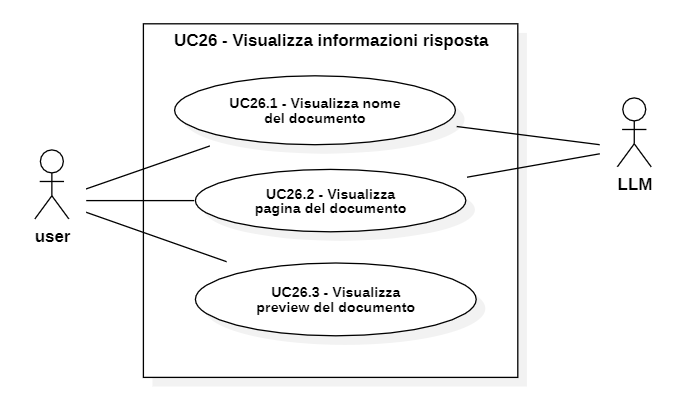
\includegraphics[width=0.9\linewidth]{UC26.1-2-3.png} %da modificare
    \caption{Diagramma UML dei casi d'uso UC-26.1, UC-26.2 e UC-26.3}
    \label{fig:UC32.1-2-3}
\end{figure}

\subsection{UC-27 Ascolta risposta}
\begin{description}
    \item[Descrizione:] L'utente vuole sentire la lettura della risposta ricevuta.
    \item[Attore primario:] Utente generico.
    \item[Attore secondario:] Modello LLM.
    \item[Pre condizioni:] Il sistema mostra la risposta ad una domanda dell'utente.
    \item[Post condizioni:] Il sistema riproduce la risposta con un audio.
    \item[Scenario:]
    \begin{enumerate}
        \item[]
        \item L’utente pone una domanda al chatbot (\textbf{UC-13}).
        \item L'utente invia la domanda al sistema (\textbf{UC-15}).
        \item L'utente ascolta la risposta ricevuta dal sistema.
    \end{enumerate}
\end{description}

\begin{figure}[H]
    \centering
    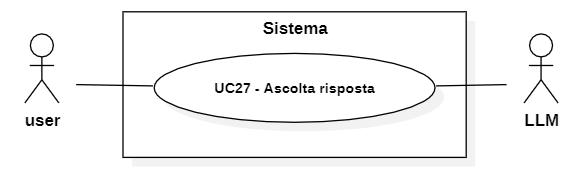
\includegraphics[width=0.9\linewidth]{UC27.png} %da modificare
    \caption{Diagramma UML del caso d'uso UC-27}
    \label{fig:UC33}
\end{figure}
